\section{Dynamic Scalable State Machine Replication}

In this section, we introduce Dynamic SSMR, discuss performance optimizations, and argue about D-SSMR's correctness.

\subsection{General idea}
\label{sec:generalidea}

S-SMR divides the state variables $v$ into $P$ partitions $\ppm_1, ..., \ppm_P$, where for each $\ppm_i$, $\ppm_i \subseteq \vvm$, and each variable $v$ in $\vvm$ has to be assigned to at least one partition and define $part(v)$ as the partitions that hold $v$. Each partition $\ppm_i$ is replicated by servers in group $s_i$. For brevity, the server $s$ belongs to $\ppm_i$ with the meaning that $s \in \ssm_i$, and say that client $c$ multicasts command $C$ to partition $\ppm_i$ means that $c$ multicasts $C$ to group $\ssm_i$.

To execute command $C$, the client multicasts $C$ to all partitions that hold a variable read or updated by $C$.
Consequently, the client must be able to determine the partitions accessed by $C$, denoted by $part(C)$. If the client cannot accurately estimate which partitions are accessed by $C$, it must determine a superset of these partitions, in the worst case assuming all partitions.
In order for clients to provide a close approximation to the command's actually accessed partitions, there is an oracle that tells the client which partitions should receive each command.

Dynamic SSMR improves on SSMR implementation by adding a central Oracle which has the information of all state variables $\vvm$, as well as provides a mechanism of controlling the access to those variable that ensure linearizability. 

We distinguish between three operation types: $read(v)$, an operation that reads the value of a state variable, $v$, $create(v, P)$, an operation that create a state variable at a specific partition P, and $move(v, \ppm_n)$, an operation that move $v$ to partition $\ppm_n$.

Consider the execution depicted in Figure~\ref{fig:read}~(a), where state variables $x$ is created on partition $\ppm_1$ in the middle of the execution of SSMR. Command $C_1(x)$ and $C_3(x)$ reads the value of $x$, $C_2(x,\ppm_1)$ create $x$ on partition $\ppm_1$. Client a first multicasts query to the $Oracle$ for location of $x$, which is not available at that time, hence $Oracle$ return empty result, which tell client a to end the execution. Client b then wants to create variable $x$ on $\ppm_1$, before sending actual creating command, client b also multicasts query to $Oracle$ to get the involved partition (eg., $\ppm_1$), then multicasts $C_2(x,\ppm_1)$ to both $Oracle$ and $\ppm_1$. Oracle will update information of $x$, and $\ppm_1$ will execute create $x$ command. From then, for every read command to $x$ (eg., $C_3(x)$), $Oracle$ could answer with partition $\ppm_1$ which is the one holds $x$.

\begin{figure*}
\begin{minipage}[b]{1.0\linewidth} % A minipage that covers the whole width of the page
\centering
      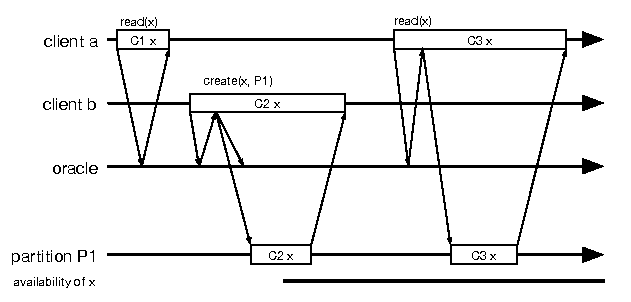
\includegraphics[width=0.6\linewidth]{figures/read_simple}
\end{minipage}
\centering
	\caption{Execution flow of D-SSMR with $create$ command}
\label{fig:read}
\end{figure*}

In the following figures~(\ref{fig:readoverlap}b, \ref{fig:readoverlap}c), where read command $C_1(x)$ comes in the middle of the execution of create command $C_2(x,\ppm_1)$, while the query of $C_1(x)$ comes after multicasts command of $C_2(x,\ppm_1)$. With the knowledge of $x$, Oracle response to the query with a positive answer, therefore there are possibilities that the read command either comes during (eg., fig.~\ref{fig:readoverlap}b) or before (eg., fig.~\ref{fig:readoverlap}c) the execution of actual write command. The SSMR model avoid the problem described in figure~\ref{fig:readoverlap}~(b) by ensuring that the execution of every command is atomic (eg., for every server $s$ in partition $\ppm$ that executes $C$, there is a server $r$ in every $\ppm' \in part(C)$ such that $delivery(C,r) < end(C,s)$. Intuitively, this condition guarantees that the execution of $C_1$ and $C_2$ at $\ppm$ overlap in time). Atomic multicast prevents the problem figure~\ref{fig:readoverlap}~(c) from happening as $deliver(C_2) \prec deliver(C_1)$, that leads to situation described in fig.~\ref{fig:readoverlap}b.

\begin{figure*}
\begin{minipage}[b]{1.0\linewidth} % A minipage that covers the whole width of the page
\centering
      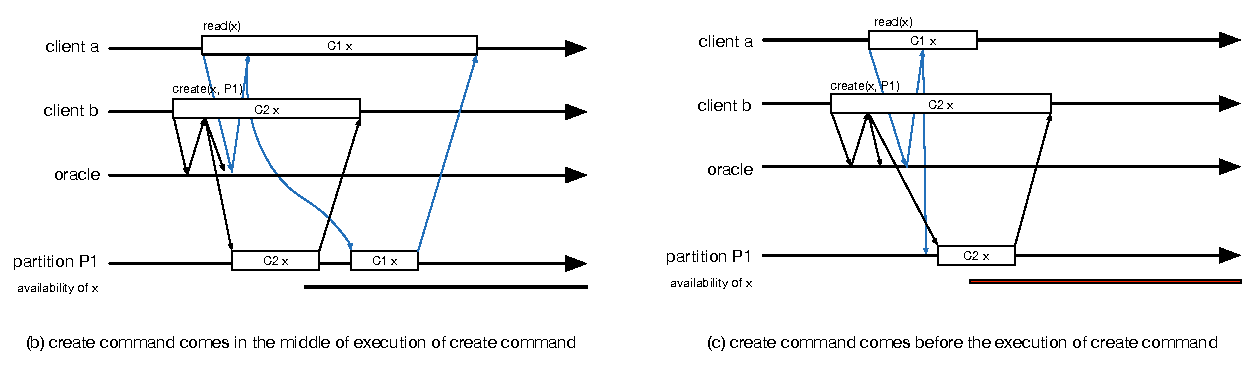
\includegraphics[width=1\linewidth]{figures/read_overlap}
\end{minipage}
\caption{Execution flow of D-SSMR with overlapping read-create commands}
\label{fig:readoverlap}
\end{figure*}


Next figure~(\ref{fig:updateoverlap} a, \ref{fig:updateoverlap} b) depicts the scenario of moving object location from a partition to another. Intuitively, the problem with the execution in fig.~\ref{fig:updateoverlap}a is that read command $C_3(x)$ executes “in between” the execution of $C_2(x,\ppm_2)$ at partitions Px and Py. Before sending $C_3$ to destination partition, client 1 send query to oracle for possible position of $x$, which is $P_1$ at that specific moment, but not correct at the execution time. In D-SSMR, we prevent that from happening by using oracle as the controller for accessing state variable on partitions, by using locking mechanism on oracle for different type of commands. Whenever a client sends a query variable's location $Q(x)$ from oracle for a command $C$, it also requires a lock $L(x)$. Then after the associated process execute command $C$, it also tell Oracle to release the lock $L$, and inform the oracle about the update of $x$ (if there is any).

There are possibilities that a client could fail in the middle of the execution of the command chains, at the moment after requires the lock and before sending the actual $C$ command to partition $P$. In this case, TODO: which one release lock, either oracle or another client that require lock again. 

\begin{figure*}
\begin{minipage}[b]{1.0\linewidth} % A minipage that covers the whole width of the page
\centering
      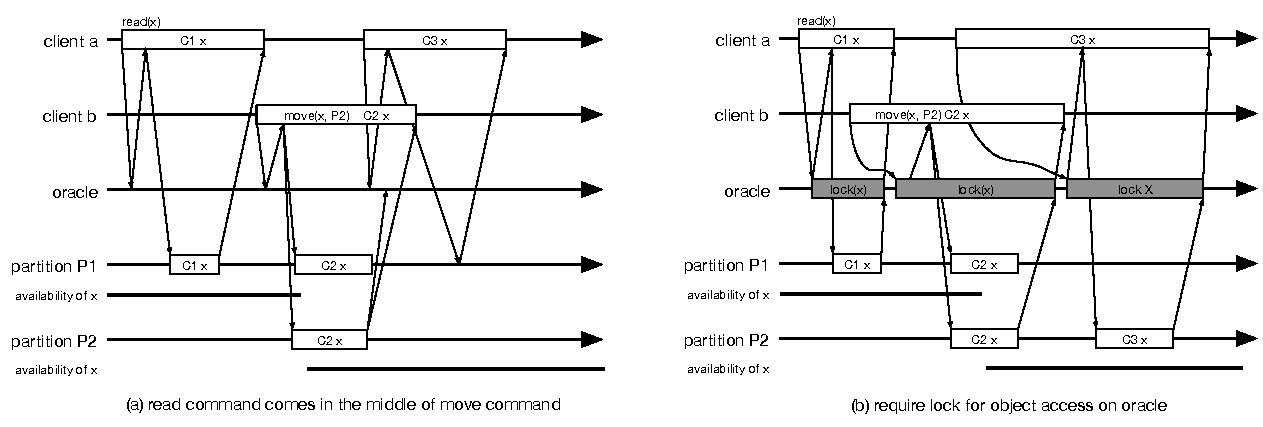
\includegraphics[width=1\linewidth]{figures/update_overlap}
\end{minipage}
\caption{Execution flow of D-SSMR with overlapping read-update commands}
\label{fig:updateoverlap}
\end{figure*}


\subsection{Detailed algorithm}
\label{sec:detailalg}

In Algorithm \ref{alg:dssmr}, we show the basic operation of D-SSMR. 
To submit a command $C$, the client queries an oracle to get set $dests$~(line \ref{algline:query_oracle}, \ref{algline:oracle_response}), which is a superset of $part(C)$ used by the client as destination set for $C$~(line \ref{algline:cli_mcast}). If the $dests$ is empty, client stop the command there. (line \ref{algline:cli_terminate})

Upon delivering $Q(C)$, oracle $O$ runs function $getPart(C)$ which returns a set $\vvm$ of involved state variables of command $C$. If there exists a variable $v_i \in \vvm$ in oracle memory, which indicates the variable $v_i$ exists on a partition $p_i \in \ppm$, oracle reply to client with $p_i$ value, or an empty result otherwise. In addition, upon delivering $C(v, \ppm)$, oracle update its memory with new location of $v$: $\vvm\_loc\{v.id\} \leftarrow \ppm$

Upon delivering $C$, server $P$ execute $C$ and reply to the client. 
% Upon delivering $C$, server $s$ in partition \pp\ multicasts $signal(C)$ to $others$, which is the set containing all other partitions involved in $C$ (lines \ref{algline:others} and \ref{algline:mcastsignals}). 
% %The purpose of $signal(C)$ is to let servers in other partitions know that there is a server in \pp\ that started executing $C$. 
% It might happen that $s$ receives signals concerning $C$ from other partitions even before $s$ started executing $C$. For this reason, $s$ must buffer signals and check if there are signals buffered already when starting the execution of $C$. For the sake of simplicity, Algorithm \ref{alg:ssmr} simply initializes such buffers as $\emptyset$ for all possible commands. In practice, buffers for $C$ are created when the first message concerning $C$ is delivered.

% After multicasting signals, server $s$ proceeds to the execution of $C$, which is a sequence of operations that might read or write variables in \vv. The main concern is with operations that read variables, as they may determine the outcome of the command execution. All other operations can be executed locally at $s$. If the operation reads variable $v$ and $v$ belongs to \pp, $s$'s partition, then $s$ multicasts the value of $v$ to the other partitions that delivered $C$ (line \ref{algline:multicastv}). The command identifier $C.id$ is sent along with $v$ to make sure that the other partitions will use the appropriate value of $v$ during $C$'s execution. If $v$ belongs to some other partition $\ppm'$, $s$ waits until an up-to-date value of $v$ has been delivered (line \ref{algline:waitvariable}). Every other operation is executed with no interaction with other partitions (line \ref{algline:executeopck}).

% After executing all operations of $C$, $s$ waits until a signal from every other partition has been received (line \ref{algline:waitsignals}) and, only then, sends the reply back to the client (line \ref{algline:sendreply}). This ensures that $C$ will be execution atomic.



% Upon delivering $C$, server $s$ in partition \pp\ multicasts $signal(C)$ to $others$, which is the set containing all other partitions involved in $C$ (lines \ref{algline:others} and \ref{algline:mcastsignals}). 
% %The purpose of $signal(C)$ is to let servers in other partitions know that there is a server in \pp\ that started executing $C$. 
% It might happen that $s$ receives signals concerning $C$ from other partitions even before $s$ started executing $C$. For this reason, $s$ must buffer signals and check if there are signals buffered already when starting the execution of $C$. For the sake of simplicity, Algorithm \ref{alg:dssmr} simply initializes such buffers as $\emptyset$ for all possible commands. In practice, buffers for $C$ are created when the first message concerning $C$ is delivered.


\begin{algorithm}
\small
%\footnotesize
\begin{distribalgo}[1]
%\STATE \textbf{Algorithm 1:\\} Scalable State-Machine Replication (S-SMR)
\vspace{1mm}

\INDENT{\emph{Initialization:}}
    \STATE  oracle: $\vvm\_loc \leftarrow \emptyset$
    % \STATE $\forall C \in \mathcal{K} : rcvd\_signals(C) \leftarrow \emptyset$
    % \STATE $\forall C \in \mathcal{K} : rcvd\_variables(C) \leftarrow \emptyset$
\ENDINDENT

\vspace{1.5mm}

\INDENT{\emph{Command $C$ is submitted by a client as follows:}}
	\STATE multicast query $Q(oracle, C)$ \label{algline:query_oracle} 
    \STATE $dests \leftarrow O(C)$ \label{algline:oracle_response} 
    \IF {$dests$ is $\emptyset$}
    	\STATE terminate $C$ \label{algline:cli_terminate}
    \ELSE
    	\STATE multicast$(dests, C)$ \label{algline:cli_mcast}
    	\STATE wait for response from one server
    \ENDIF
%    \COMMENT{$oracle(C)$ returns a superset of $part(C)$}
\ENDINDENT

\vspace{1.5mm}

\INDENT{\emph{Command $C$ is executed by a oracle as follows:}}
	\INDENT{\textbf{upon} deliver $Q(C)$}
		\STATE $v \leftarrow get part(C)$
		\IF {$v$ in $\vvm\_loc$}
			\STATE send reply to client $\vvm\_loc\{v.id\}$
		\ELSE
			\STATE send reply to client $\emptyset$
		\ENDIF
	\ENDINDENT

	\INDENT{\textbf{upon} deliver $C(v, \ppm)$}
		\STATE $\vvm\_loc\{v.id\} \leftarrow \ppm$
	\ENDINDENT

\ENDINDENT

\vspace{1.5mm}
\emph{TODO: Should give the detail algorithm of SSMR? or give short description of dssmr}
\vspace{1.5mm}

\INDENT{\emph{Command $C$ is executed by a server in partition \pp\ as follows:}}
	\INDENT{\textbf{upon} deliver$(C)$}	    
		\STATE execute $op$ \label{algline:executeopck}
		\STATE send reply to client \label{algline:sendreply}
	\ENDINDENT
\ENDINDENT

% \INDENT{\emph{Command $C$ is executed by a server in partition \pp\ as follows:}}
% 	\INDENT{\textbf{upon} deliver$(C)$}
% 	    \STATE $others \leftarrow dests \setminus \{\ppm\}$ \label{algline:others}
% 	    \STATE multicast$(others, signal(C))$ \label{algline:mcastsignals}
% 		\FOR{each operation $op$ in $C$}
% 			\IF{$op$ is $read(v)$}
% 			    \IF{$v \in \ppm$}
% 			        \STATE multicast$(others, \{v,C.id\})$ \label{algline:multicastv}
% 			    \ELSE
% 			        \STATE \textbf{wait until} $v \in rcvd\_variables(C)$ \label{algline:waitvariable}
% 			        \STATE update $v$ with the value in $rcvd\_variables(C)$
% 			    \ENDIF
% 			\ENDIF
% 			\STATE execute $op$ \label{algline:executeopck}
% 		\ENDFOR
% 		\STATE \textbf{wait until} $rcvd\_signals(C) = others$ \label{algline:waitsignals}
% 		\STATE send reply to client \label{algline:sendreply}
% 	\ENDINDENT
	
% 	\vspace{2.0mm}
% 	\INDENT{\textbf{upon} deliver$(signal(C))$ from partition $\ppm'$}
% 	    \STATE $rcvd\_signals(C) \leftarrow rcvd\_signals(C) \cup \{\ppm'\}$
% 	\ENDINDENT

% 	\vspace{2.0mm}
% 	\INDENT{\textbf{upon} deliver$(\{v, C.id\})$}
% 	    \STATE $rcvd\_variables(C) \leftarrow rcvd\_variables(C) \cup \{v\}$
% 	\ENDINDENT
			
% \ENDINDENT

\vspace{1.5mm}
%\vspace{2mm}

\textbf{Algorithm variables:}

\vspace{1mm}

$\vvm\_loc$: the set of locations of all state variables in the system.

\vspace{1mm}

$Q(oracle, C)$: multicast command to oracle for querying involved partition of command C

\vspace{1mm}

$O(C)$: response of oracle that returns a superset of $part(C)$

\vspace{1mm}

$dests$: set of partitions to which $C$ is multicast

\vspace{1mm}

$C(v, \ppm)$: command that create variable $v$ in partition $\ppm$

% \vspace{1mm}

% $others$: set of partitions waiting for signals and variables from \pp; also, \pp\ waits for signals from all such partitions

% \vspace{1mm}

% $signal(C)$: a synchronization message that allows S-SMR to ensure $C$ to be execution atomic

% \vspace{1mm}

% $rcvd\_signals(C)$: a set containing all partitions that already signaled \pp\ regarding the execution of $C$

% \vspace{1mm}

% $rcvd\_variables(C)$: a set containing all variables that must be received from other partitions in order to execute $C$

\caption{Dynamic Scalable State-Machine Replication (D-SSMR)}
\label{alg:dssmr}
\end{distribalgo}
\end{algorithm}

\subsection{Performance optimizations}
\label{sec:optm}
TODO: add content, talk about caching

Algorithm 1 can be optimized in many ways. In this section, we briefly mention some of these optimizations and then detail caching.

\begin{figure*}
\begin{minipage}[b]{1\linewidth} % A minipage that covers the whole width of the page
\centering
      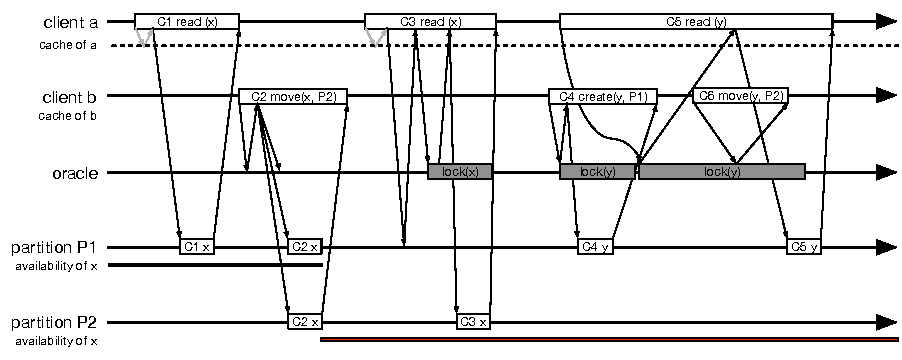
\includegraphics[width=0.85\linewidth]{figures/cache}
\end{minipage}
\caption{Execution flow of D-SSMR with oracle caching on client}
\label{fig:cache}
\end{figure*}


\subsection{Correctness}
\label{sec:correctness}
TODO: add content